\subsubsection{Introduction of CHIL Environment}
\paragraph{Digital Real-Time Simulator (DRTS)}
RT-LAB real-time simulator is used for real-time simulation of MVDC power system which uses MATLAB/Simulink platform for modeling the system. The system modeled in Simulink is converted to C code and loaded in DRTS for real-time execution of the system. Both digital and analog inputs and outputs (I/O) interfacing facilities are available with the real-time simulator to communicate with external devices. The Target computer (real-time simulator) uses TCP/IP network to communication with the Host computer. REDHAT real-time operating system is used to run the target computer. RT-LAB uses advanced computational techniques and fixed time-step solvers designed for                 real-time simulation which is known as ARTEMIS \cite{mikkili2015review}. 

   
{\textbf{OP7020: }}The OP7020 is an expansion unit for the RT-LAB simulator and it contains a Xilinx Virtex-7 FPGA. To communicate with other FPGA devices (for examples OP7000 and OP5607) or external controllers, it has 16 high-speed fiber optic links using Small Form-factor Pluggable (SFP) transceivers. It follows Aurora (1 to 5 Gbits), Gigabit Ethernet (1 Gbit) protocols. The custom protocol can be also implemented. In order to connect OP7020  with the Target computer (Opal-RT simulator), high speed (30Gbps) fiber-optic X4 links are available \cite{FPGA_EXP}. 


{\textbf{OP5607: }}The OP5607 is an expansion unit available for the Opal-RT simulator. It has a Xilinx Virtex-7 FPGA. It also has 8 signal conditioning and analog/digital converter modules with 32 digital and 16 analog channels. Which supports 256 digital and 128 analog signals. To connect with other devices (OP7020 and OP4500) and external controllers, 16 high speed (speed from 1 to 5Gbps) SFP multi-mode fiber optic links are interfaced with OP5607.  It follows Aurora (1 to 5 Gbits), Gigabit Ethernet (1 Gbit), and customer requirements based protocols \cite{FPGA_EXP}. In the front side of the OP5607, there are mini-BNC terminals for monitoring signals through an oscilloscope. It has high speed (30Gbps) PCI Express gen2 x4 fiber-optic links to interface with the Target computer (Opal-RT simulator). 

\subsubsection{CHIL Simulation Interfacing}
Fig. \ref{ch5_f111} shows the block diagram of the CHIL simulation setup. The Host computer (not shown) is an Intel core i7, 3.2GHz processor and it is connected to the Target-real time simulator via Ethernet cable. Four different cores of the real-time simulator are used to load and run four different subsystems of the loads, sources, battery and supercapacitor. The available Xilinx System Generator (XSG) and RT-XSG library are used to model the FL controller based ESM system. RT-XSG library is also used to configure the analog outputs in OP5607. The Xilinx System Generator is used to compile the model into FPGA bit streams. The bit stream file of the FL based ESM system controller is implemented in the FPGA board available with OP7020. The OP5607 is used to produce analog output signals by loading the analog output configuration bit stream file in OP5607. The target computer (real-time simulator) is connected to the OP5607 and OP7020 via fiber-optic PIC express links. 


Fig. \ref{ch5_f112} shows the experimental setup for the CHIL based test system. Fig. \ref{ch5_f112a} shows the front panel. Where the top FPGA board, OP7020 is used to implement the FL based ESM controller for CHIL based testing. From Fig. \ref{ch5_f112b}, the bottom board is OP5607 and it is connected to the scope to show the analog output results. The top FPGA board (OP7020) works as a master and bottom FPGA (OP5607) board works as a slave. A black audio cable is used for synchronization between them. There are quick monitoring ports on the front panel of OP5607. The RJ45 connector (white cable) connects analog/digital ports of OP5607 to quick monitoring ports. Eventually, analog output signals are passed from the quick monitoring ports to the oscilloscope through the BNC connectors.  Fig. \ref{ch5_f112b} shows the back panel. From Fig. \ref{ch5_f112b}, the orange cables are fiber optic PCI express cables which connect OP5607 and OP7020 to the real-time simulator.

\begin{figure}[h!]
\centering
%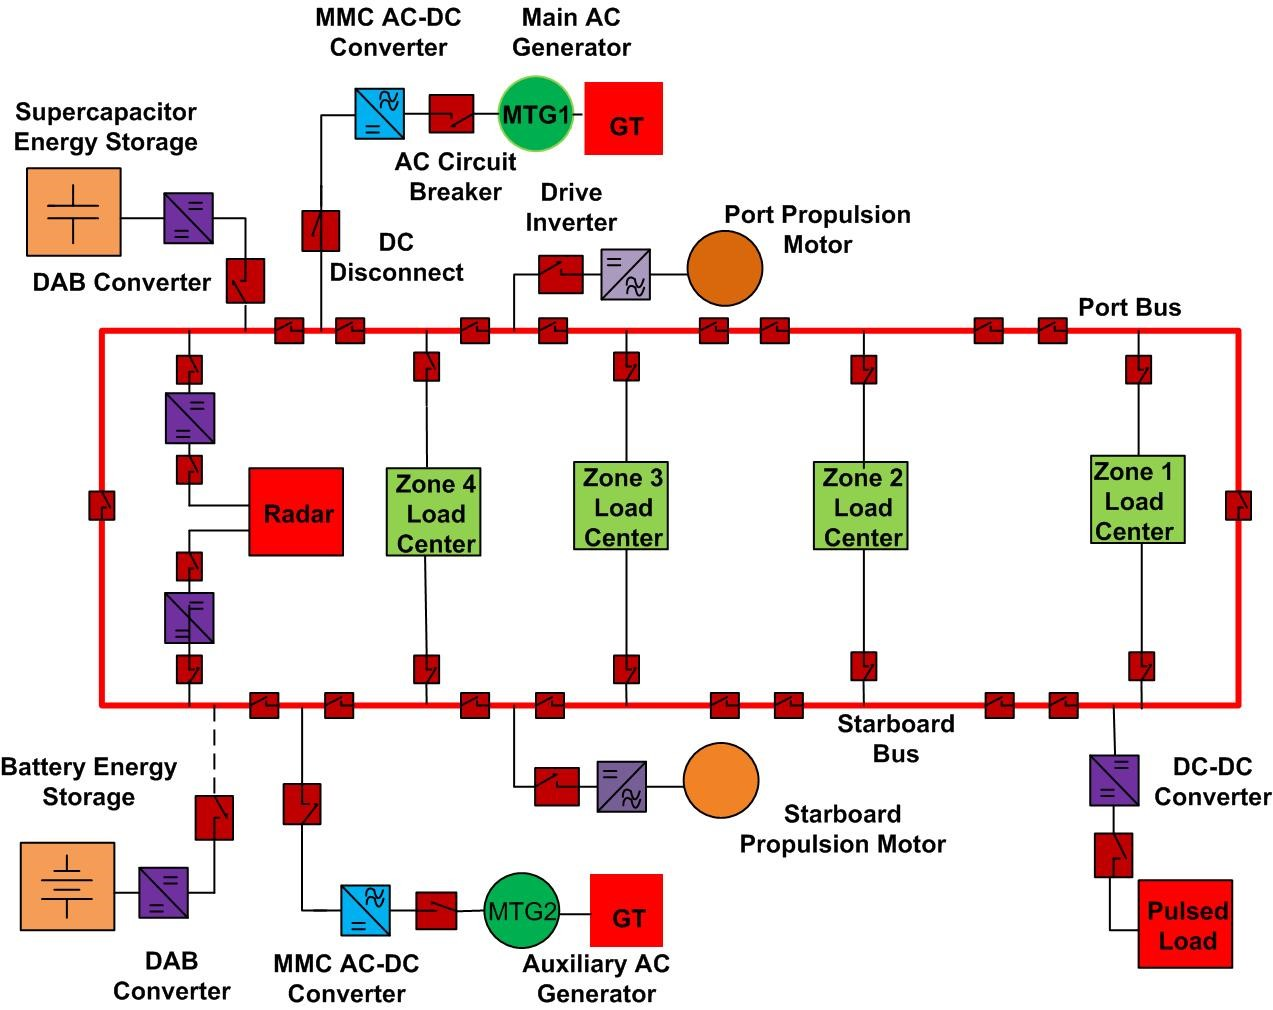
\includegraphics[width=\columnwidth]{f1}

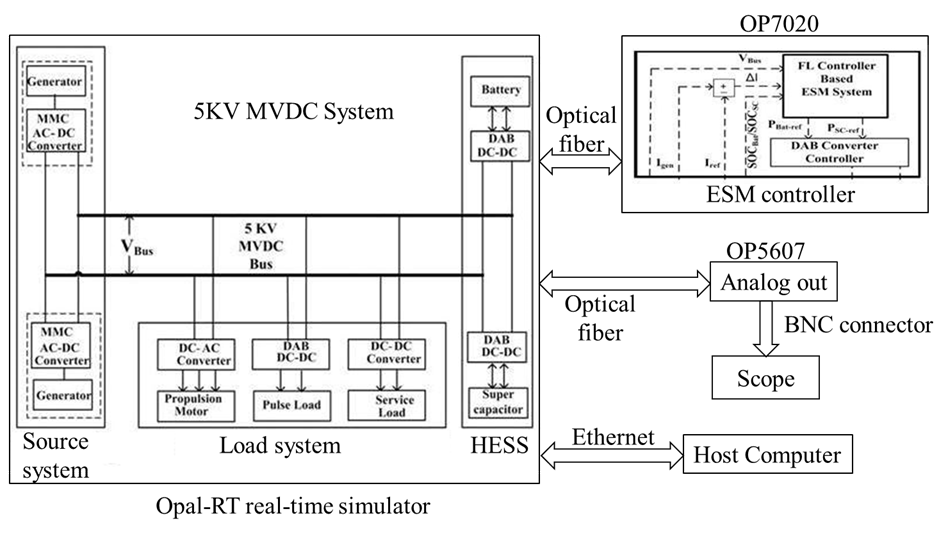
\includegraphics[width=3.5in]{f1111}
\caption{Hardware setup block diagram for CHIL simulation of FL based ESM system.}
\label{ch5_f111}
\end{figure}

\begin{figure}[ht!]
\begin{subfigure}{1\columnwidth}
\begin{center}
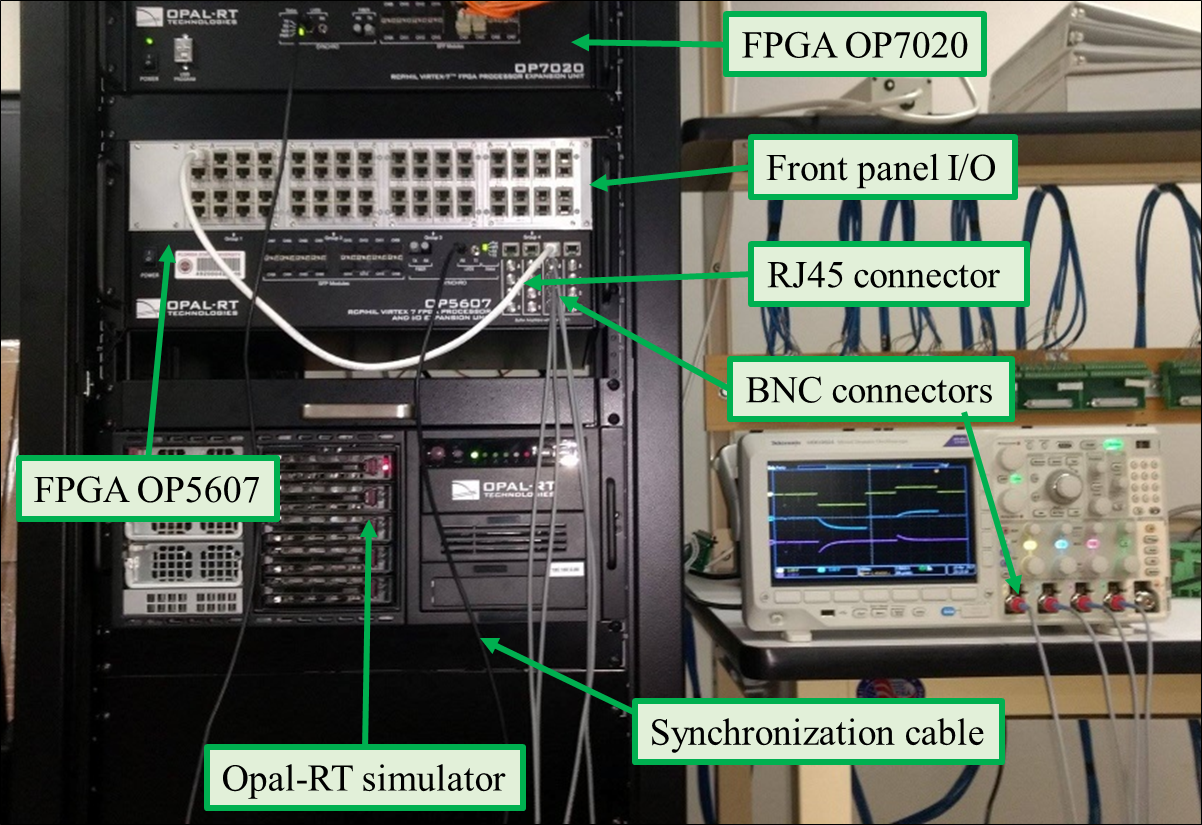
\includegraphics[height=1.9in, width=3.46in]{f112a}
\end{center}
\caption{Front panel.}
\label{ch5_f112a}
\end{subfigure}
\begin{subfigure}{1\columnwidth}
\begin{center}
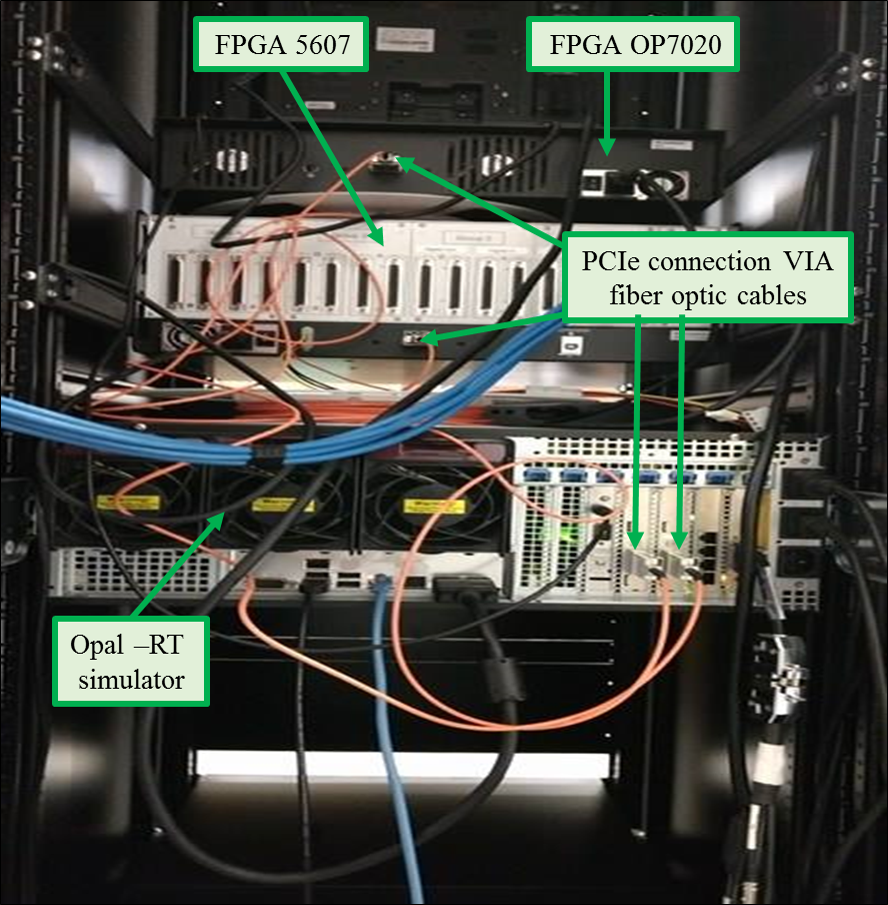
\includegraphics[height=2.05in, width=3.46in]{f112b}
\end{center}
\caption{Back panel.}
\label{ch5_f112b}
\end{subfigure}
\caption{Experimental setup for CHIL operation of FL based ESM system.}
\label{ch5_f112}
\end{figure}
